% !TEX encoding = System
\documentclass{noithesis}

\usepackage{algorithm}  
\usepackage{algorithmicx}  
\usepackage{algpseudocode}  
\usepackage{amsmath}  
\usepackage{float}
\begin{document}

%% 论文开始

\title{《图上的游戏》命题报告}
\author{华东师范大学第二附属中学~~左骏驰}

\maketitle

\begin{abstract}
本文将介绍作者在某次省选训练时为几个学校命制的一道交互题。题目深度挖掘了有关图的连通性、图的生成树、有根树的DFS序的知识,并有机地结合了二分查找、分治的基本算法,以及随机化的思想。本题所用的知识点并不高级,但需要选手对基本算法蕴含的重要思想有深刻的理解。

此外,本题的部分分很多,能引导选手走向正解,且区分出拥有不同思考程度的选手。正解大概分为三个部分,而想到每一部分都会有相应的分数。

本文提出一种命题上的目标:部分分的设计与正解高度契合。
\end{abstract}

\section{试题大意及数据范围}

\subsection{题目描述}


小 Z 有一张 $n$ 个点 $m$ 条边的可能有重边,但没有自环的无向图。小 U 想要知道这张图的样子,但小 Z 不肯告诉
它。

小 Z:我可以告诉你这张图是连通的,点从 $0$ 标号至 $n - 1$,边从 $0$ 标号至 $m - 1$。

小 U:好那删去一条边后,这张图的连通状况如何呢?

小 Z:反正你也猜不出来,就这样吧。你每次告诉我一个边的编号的集合 $S$,再给定一个点 $u$,然
后我可以帮你计算把编号在 $S$ 中的边连接后,$0$ 号点与点 $u$ 是否连通。

听到小 Z 的这句话后,小 U 苦思冥想,仍然不知道如何才能问出这张图的每条边到底连接哪两个
端点。

因此他找到了你,想让你帮他问出这张图的信息。我们保证这张图是预先生成的,也就是说不会随
小 U 的询问而改变。并且你不能询问太多次,你需要在 30000 次内得到这张图的信息!

\subsection{交互方式}

你不需要实现主函数,你只需实现一个函数:

\lstset{language=C}
\begin{lstlisting}
std :: vector<std :: pair<int, int> > solve (int n, int m) ;
\end{lstlisting}

这个函数应该返回一个长度为 $m$ 的数组 $e$,其中 $e[i]$ 表示第 $i$ 条边连接的两个端点(顺序无关)。

同时,你需要在你提交的文件 $graph.cpp$ 中包含 $graph.h$ 头文件,
我们下发了 $sample\_graph.cpp$供你做参考。

你所实现的这个函数只能调用交互库中的函数:

\lstset{language=C}
\begin{lstlisting}
bool query (int u, std :: vector<int> s) ;
\end{lstlisting}

这个函数中 $u$ 是一个 $[0, n - 1]$ 中的整数,$s$ 是一个长度为 $n$ 的 int 数组,且值只能为 $0$ 或 $1$。若
$s[i] = 1$,则表示 $i$ 是否在小 U 所询问的集合 $S$ 中, 否则表示不在集合 $S$ 中。这个函数的意义是给定 $u$ 和 $S$,询问 $0$ 号点能否通过编号在 $S$ 中的边到达 $u$。

\subsection{题目数据范围及特殊限制}

对于所有数据,保证$1 \leq n, m \leq 600$,图是连通图。

Subtask 1(6 pts): $n, m \leq 25, m = n - 1$。

Subtask 2(10 pts):$n, m \leq 25$。

Subtask 3(17 pts): $m = n - 1$,且图中每个顶点的度数$\leq 2$,$0$号点的度数为$1$。

Subtask 4(24 pts):$m = n - 1$。

Subtask 5(19 pts):保证将编号$< n - 1$的边提出后,编号为$i$的边所连接的两个顶点为$i, i + 1$。

Subtask 6(13 pts):保证将编号$<n - 1$的边提出后,图构成一棵树。

Subtask 7(11 pts):无特殊限制。

\section{前置技能}

\subsection{图的基本概念及术语}
对于一个无向图$G$,如果任意两个顶点之间均存在一条路径连接这两个顶点,就称该图为\textbf{连通图}。

若图$G$满足任意两个顶点之间有唯一的一条路径与它相连,则称$G$是\textbf{树}(或称无根树)。

对于一般的无向连通图$G$,若树$T$的点集与$G$相同且边集是它的子集,则称$T$是$G$的\textbf{生成树}。

给一棵无根树规定了一个根后,就形成了一棵有根树。每个非根顶点$u$到根的路径上第一个(不含起点)的顶点称为$u$的\textbf{父亲}。如果$v$为$u$的父亲,则称$u$是$v$的\textbf{儿子}。如果某个顶点不存在儿子,则称这个顶点为\textbf{叶子}。我们再把所有根到顶点$u$路径上的点成为$u$的\textbf{祖先}。对于一个特定的顶点$u$,我们把去掉$u$到它父亲的边(如果存在的话),$u$能到达的点的集合称为$u$的\textbf{子树}。

此外,如果某棵有根树$T$满足$T$的每个顶点的儿子个数$\leq 1$,则称$T$为\textbf{链}。

图$1$是一个有根树的例子,其中$0$有两个儿子$1, 2$,$1$有两个儿子$3, 4$,$2$有$5$这一个儿子,且$3, 4, 5$没有儿子,它们是叶子。

图$2$表示的是链。其中$0, 1, 2, 3, 4$恰好有$1$个儿子,$5$是叶子。

\begin{figure*}
\centering
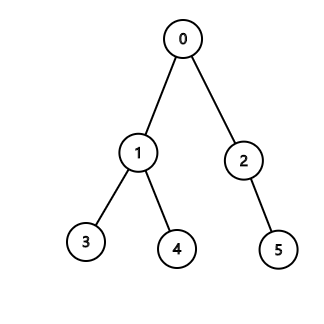
\includegraphics[scale=0.45]{graph2.png}
\caption{以$0$为根的有根树的一个例子}     \label{fig:ss}
\end{figure*}

\begin{figure*}
\centering
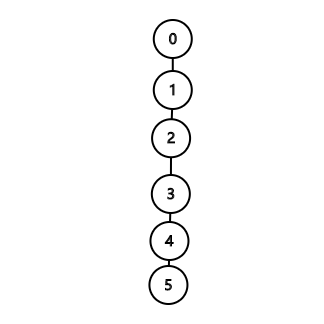
\includegraphics[scale=0.45]{graph4.png}
\caption{以$0$为根的链的一个例子}     \label{fig:ss}
\end{figure*}

\subsection{树的dfs序}

对于一棵从$0$开始标号的有根树$T$,我们有一个常见的dfs算法如下。

\begin{algorithm}  
    \caption{树上的dfs算法} 
        \begin{algorithmic}[1]
        \State $Ans \gets \emptyset$
        \Function {dfs}{$u$}  
            \State $Ans \gets Ans \cup \{ u \}$
            \For{$v$ in $child(u)$}
                    \State dfs(v)
            \EndFunction  
        \end{algorithmic}
\end{algorithm}

上述伪代码中$child(u)$表示$u$的儿子的某个序列。

运行该dfs算法后,$Ans$会返回$dfs$过程中构成的序列。
我们记$u$在dfs序中的位置(从$0$开始标号)为$id_u$,那么我们有这么如下性质:

\textbf{性质1}:若$v$是$u$的祖先,则$id_u \ge id_v$。

\textbf{性质1证明}:在dfs访问过程中,若访问了某个顶点,则其父亲也必定被访问,故$id_u \ge id_v$。



\subsection{一个基本方法}

我们来考虑这样一个简单的问题。$1, 2, \cdots, N$中有$M$个数是好的(这这里我们认为$M$比较小,$N$比较大)。现在你可以指定一些数,询问在这些数里面是否有好数,你需要用$O(M \log N)$次操作来找到所有好数。这一思想在这一交互题中用到了很多次,也在OI比赛很多的交互题上都有用。

我们采用分治的思想。伪代码如下:(这里Ask(S)的返回值表示$S$中是否存在好数,$Ans$最终会得到所有好数的集合。)

\newpage

\begin{algorithm}[h]
  \caption{一个找到所有好数的方法}
  \begin{algorithmic}
  \State $Ans \gets \emptyset$
  \Function {solve}{left, right}
    \State $mid \gets (left + right) / 2$
    \If {$left = right$}
        \State $Ans \gets Ans \cup \{ mid \}$
    \Else
        \State $S_1 \gets \emptyset$
        \State $S_2 \gets \emptyset$
        \For{$i = left$ to $mid$}
            \State $S_1 \gets S_1 \cup \{ i \}$
        \EndFor
        \For{$i = mid + 1$ to $right$}
            \State $S_2 \gets S_2 \cup \{ i \}$
        \EndFor
        \If {$Ask(S_1)$}
            \State solve(left, mid)
        \EndIf
        \If {$Ask(S_2)$}
            \State solve(mid + 1, right)
        \EndIf
    \EndIf
  \State solve(1, N)
  \end{algorithmic}
\end{algorithm}




考虑这个算法所构成的分治树的结构。它的叶子的区间长度为$1$,且这个区间内的数必定为好数。每个叶子的深度为$O(\log N)$,故分治树总节点数是$O(M \log N)$的。这样询问的次数也是$O(M \log N)$的。

\section{算法介绍}

我们将所要介绍的算法将顺着部分分的提示逐步深入,因此我们将按照链、树、连通图的顺序介绍。

\subsection{链}

这个部分分有很多种$O(n \log n)$做法,基本都借鉴了随机化的思想。

这里我们给出一种做法。

首先将点 $\{ 1, 2, \cdots, n - 1\}$随机排列为$p_1, p_2, \cdots, p_{n - 1}$。然后依次加入每个点$p_i$,我们需要维护:

1. 已经加入的点之间的相对顺序

2. 对于每条边,在它的左侧(就是靠近$0$号点的一侧)的所有点的集合。

(初始时我们认为$0$号点在最左侧,且我们加入一个在最右侧的虚拟节点$n$号点)

那么我们对于新加入的每个点$p_i$,可以先在原序列上二分出来它要插入到已加入顶点的哪个位置。这一步具体可以保留在某个点左侧的边,然后判断 0 能否到达新加入的点,来缩小插入到的顶点的范围。

接下来我们在插入的两个点$u_l, u_r$之间的边中,暴力地对每一条边$e$判断它在$p_i$的左边还是右边。这一步我们可以通过删去这条边保留其它所有边,判断$0$是否与$p_i$连通来实现。

接下来我们来大致说明其复杂度为$O(n \log n)$。

由于每次二分的复杂度已经是$O(n \log n)$了,只需研究暴力判断每一条边的位置的复杂度。假设已经加了$i$个点,那么在随机意义下需要花费的代价是$O(\frac{n}{i})$的!而$\sum_{i = 1}^{n + 2} \frac{1}{i} = O(\ln n)$,故$\sum_{i = 1}^{n + 2} \frac{n}{i} = O(n \ln n)$。得到总复杂度为$O(n \log n)$。

于是我们在 $O(n \log n)$ 的询问次数内解决了这个子问题。


\subsection{树}

以下均把树看成是以 0 为根的有根树。

\subsubsection{$O(n^2)$做法}

对于每条边$e_i$我们把这条边删去,保留其它所有边。然后逐次询问$0$号点能够到哪些点。那些不能到达的点就构成了某个点的子树。

反过来,我们也可以直到每个点到它的根上的所有边,这样也就知道了每个点的深度。

然后对每条边,我们找删去它,根不能到达的点中深度最小的点,这就是\textbf{子树的根},也是\textbf{这条边上的较深}的端点。

之后对每个点$u$,我们来找包含它的子树大小最小的子树(不包括$u$本身的子树),就可以得到它的父亲了。

最后,我们就可以从每条边的一个较深端点推到两个端点,就解决了这一问题。

而我们一共要删去$n - 1$条边,每条边询问$n - 1$次,因此总复杂度为$O(n^2)$。


\subsubsection{将边分割为链的做法}

\newpage

\begin{figure*}
\centering
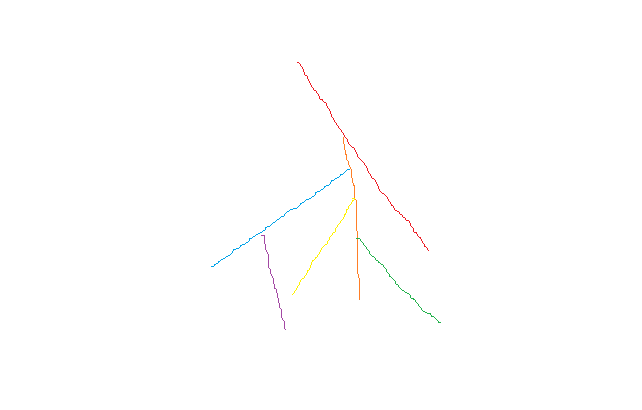
\includegraphics[scale=0.45]{graph5.png}
\caption{}     \label{fig:ss}
\end{figure*}

我们考虑把每条点标一个数$0, 1, \cdots, c - 1$,使得标同一种数的点构成了一条链,且每条链的顶端的父亲所在的链的标号比它小。一开始所有树上的边都是未标记的。

图$3$是正确的划分方法的一个例子。其中红所在链的每条边的较深端点和根标号为$0$,橙色链标号为$1$,黄色链标号为$2$,绿色链标号为$3$,蓝色链标号为$4$,紫色链标号为$5$。对这种分割方法的直观理解是:后面的链都“接在”前面某条链之下。这使得我们之后只需要对每一条链分别求解,再找到每条链和之前部分的“拼接点”!


固定一个顶点$u$,定义所有$0$到$u$路径上的\textbf{未标记的边为好边}。如果一次题目中询问的集合的补集包含了\textbf{好边},则$0$到$u$就不连通了。

依次考虑$1, 2, \cdots, n - 1$这些点。

情形一:只保留已经标记的边,$0$ 就与 $u$ 连通。这说明 $u$ 本身在原先的某条
链上,那么我们可以保留两个端点所在链的编号 $\leq mid$ 的边,询问 $0$ 是否与 $u$
连通,通过二分可以知道 u 所在的链的编号了。

情形二:只保留已经标记的边,$0$ 不与 $u$ 连通,这个时候我们找到 \textbf{所有未标记的好边}。这一步可以用2.3中的那个分治的方法来实现。最后我们让这些边所在的较深的点变为一条编号为$c$的新的链,然后令新的$c$为$c + 1$。

注意到碰到情形二的时候,你可以知道新开的一条链的点连向它父亲的边的编号的集合,但是你不知道这条链上有哪些点。然而你可
以在之后通过情形一的做法来确定这条链上的所有点。

因此在最后,我们可以知道每条链上有哪些点,还知道这些点连向它父亲的编号的集合。

\subsubsection{分割为链之后的方法}

如果知道了这些,我们可以按照标号从小到大的顺序依次确定每条链的顺序,每条链上的每个点连到它父亲的边的编号,这一步直接使用链的部分分
做法即可。所以我们只需要知道每条链的顶端的父亲的点的编号。

这一步可以使用在 dfs 序上二分的做法。具体来说就是假设你当前加入
的这条链标号为 $i$,所有标号 $<i$ 的点构成的树 $T$ 是已知的,只是从 $i - 1$ 到 $i$ 的这条边未知。然后你对 $T$ 保留端点的 dfs 序 $\leq mid$ 的边,再保留这
条链顶端到它父亲的边的编号,询问保留这些边能否到达链顶端的点,就可以知道这条边的父亲的 dfs 序是否 $\leq mid$。

注意到这里我们用到了$2.2$的性质一,这一性质保证了把两个端点的dfs序都$\leq mid$得边保留后,得到的子图连通了所有$dfs$序$\leq mid$的顶点。

\subsection{连通图}

\subsubsection{找生成树的$O(nm)$算法}

我们只需找出一个边的下标的集合,使得这些下标的边构成了一棵生成树。这样就可以套用找树的所有方法了。

一开始,所有边都是未标记状态。然后依次加入$1, 2, \cdots, n - 1$号顶点。假设加入到了顶点$u$,且之前标记的边连通了$0$和$1, 2, \cdots, u - 1$。


\textbf{性质一}:依次扫描所有未标记的边,若这条边删去后$0$就不能到达$u$,就把它变为标记的边,否则就跳过这条边。则我们这样得到的新的标记的边能够连通$0$和$u$,且被标记的边仍然构成森林。

\textbf{性质一证明}:

由于一开始图是连通的,显然$0$能够到达$u$,且
我们考虑依次扫描所有未标记的边,跳过一条边并不影响$0$到$u$之前的连通性。

再证明得到的新的被标记的边构成的子图无圈。反证法,假设存在一个圈$C$,它由$e_{i_1}, e_{i_2}, \cdots, e_{i_l}$构成,其中$i_1 < i_2 < \cdots < i_k$为它的标记时间。
则在标记$i_1$的时候,$i_1$的两个端点由$e_{i_2}, e_{i_3}, \cdots, e_{i_k}$这些边连通了。因此删去$e_{i_1}$不影响连通性,也就是说$e_{i_1}$不是桥,故$e_{i_1}$应该跳过,而不是被标记,矛盾!



通过性质一,我们就可以每一轮$O(m)$地把连接$0, 1, \cdots, u - 1$的森林扩充为$0, 1, \cdots, u$的生成森林,进而在$O(nm)$的询问次数解决了找生成树的方法。

\subsubsection{找生成树的$O(n \log m)$算法}

注意到最后我们只需要标记$n - 1$条边,我们不妨把前一个算法的依次扫描的过程改成\textbf{每次找一个最大的前缀删去,使得$0$仍然能够到达$u$}。这一过程可以用简单的二分查找来实现。

这样依次二分下一条需要标记而不是被删除的边,一共进行$n$轮二分操作,每一轮二分操作除了最后一次二分之外,其余的二分操作都会使得我们多标记了一条边,所以最多$n + n - 1 = O(n)$次二分操作。总时间复杂度$O(n \log m)$。

\subsubsection{找非树边的方法的$O(nm)$算法}

首先套用树的算法,可以找出其生成树$T$的每一条边连接的两个点了。

对于每条树边$(u, v)$,设$u$是其中较深的顶点。假设我们要询问的边是$e_i = (w_1, w_2)$,其中$w_1, w_2$未知。我们把$(u, v)$删去,保留其余所有边,再保留$e_i$,询问$0$是否和$u$连通。这样若答案为连通,就说明$w_1, w_2$中恰有一个在$u$的子树内(这种情况如图$4$所示),也就是说$w_1 \rightarrow w_2$在$T$上的路径经过了$(u, v)$。

对每条非树边,我们可以依次得到每条树边是否在它“跨过”的路径上。这样就可以从路径的端点推出$w_1, w_2$了!

\begin{figure*}[htbp]
\centering
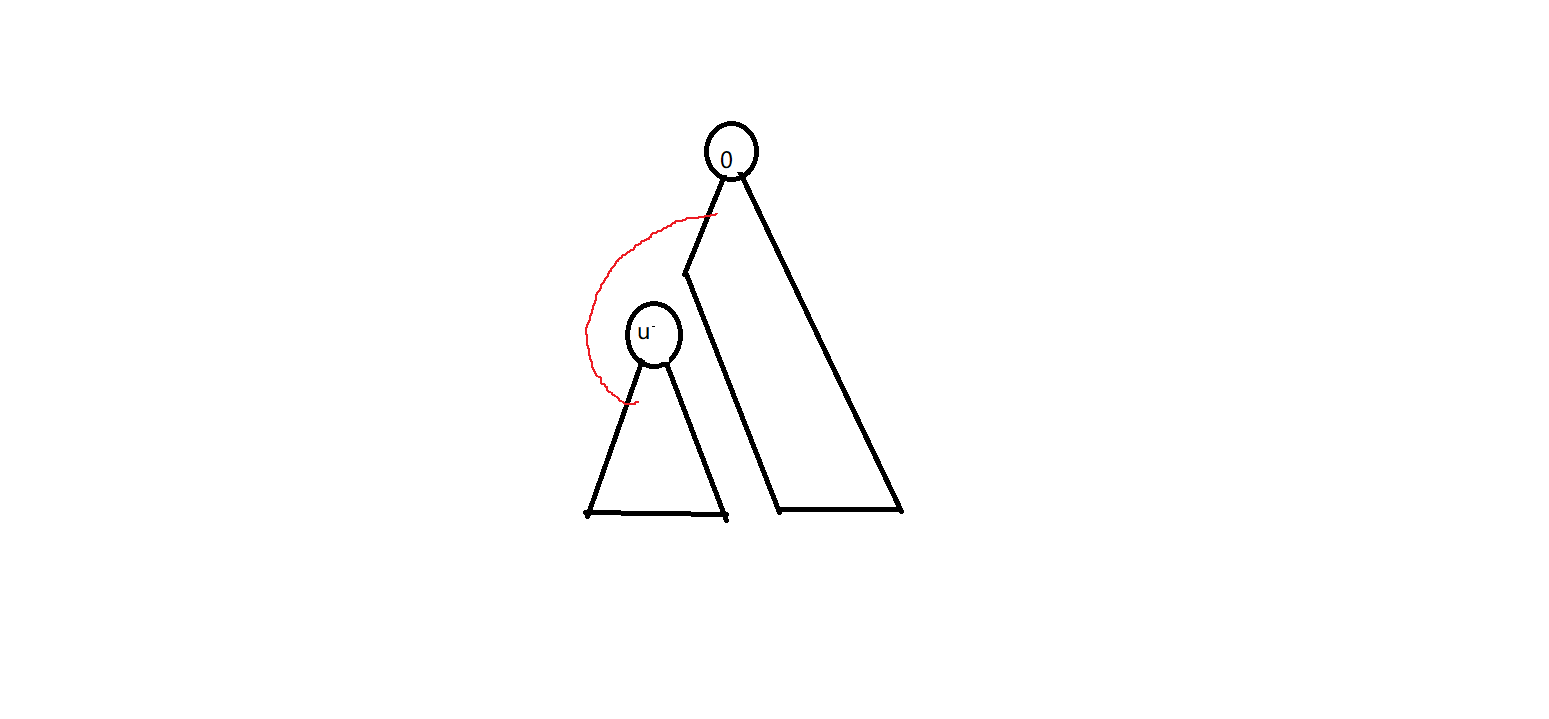
\includegraphics[scale=0.45]{graph6.png}
\caption{其中红边代表我们未知的一条非树边}     \label{fig:ss}
\end{figure*}

\newpage

\subsubsection{找非树边的$O(m \log m)$算法一}


这个部分可以自顶向下做,也可以自底向上做。由于自底向上常数稍小,易于理解,我们就先写这种做法了。

考虑删去一个生成树的叶子 u,在删去的同时你需要知道与 u 相连的所有边,在把所有点删去后所有非树边就可以得到了。


第一步:我们称和$u$相邻的边为好边。把$T$上和$u$相邻的唯一一条边删去,如果某次询问包含了所有$T$的其它$n - 2$条边和一条好边,$0$就与$u$连通。如果只包含$T$的其它$n - 2$条边,而没有包含好边,就不与$u$连通。我们再次套用之前找好数的方法,即可找到所有好边的\textbf{下标}。


第二步:对每条非树边找到另一个端点。这一步可以用之前说过的在dfs序上二分的思路去实现。具体来说,保留端点dfs序$\leq mid$的顶点,和你要考虑的那条非树边$e_i$,如果$0$此时能够到达$u$,说明$e_i$的另外一个端点dfs序$\leq mid$,否则就$> mid$。这样我们就可以二分出这条连接叶子的非树边的另外一个端点了。


最终,我们用 O(m log m) 的询问次数解决了此题。

\subsection{找非树边的$O(m \log m)$算法二}

我们按照任意的顺序考虑每条树边。如果我们考虑到了一条树边$(u, v)$(设$v$是$u$的父亲),删除后形成了两个连通块$C_1,C_2$,则我们要找到所有跨过$C_1, C_2$的非树边。

初始时将所有非树边标记为“未知的”。每次删去\textbf{恰好$(u, v)$这一条边},保留其它的\text{$n - 2$条树边},若我们再加上的非树边中存在好边,$0$就和$u$连通,否则$0$就和$u$不连通。因此我们又可以用前文所述的分治的方法找到所有\textbf{未知的好边}。把这些好边标记为\textbf{已知的},再之后不必考虑它们。

接下来对于某条找到的非树边$e$,我们再把$C_1$这棵子树内的顶点按dfs序标号,然后保留端点dfs序$\leq mid$的边,保留$C_2$内所有树边,保留$e$,询问$0$是否可以到达$u$,若可以,则说明在$C_1$的端点的其dfs序$\leq mid$,否则就$> mid$。同样地,我们对连通块$C_2$也做一样的事情,就可以知道这条非树边$e$的两个端点了。

在考虑完$n - 1$条边后,我们即可得到所有的树边了(因为每条非树边都必定“跨过”至少一条树边)。

注意到其实算法一是算法二在特殊的考虑边的顺序下变化出的算法。如果我们把算法二中考虑边的顺序变成:每次逐渐剥去一个叶子与它父亲相连的边,就相当于算法一了。然而剥叶子的时候,我们每次“好边”的一个端点是固定的,可以把两次dfs序上二分改成一次dfs序上二分,因此减少了常数。


\section{命题过程}

这一问题是笔者在试图命制一道树上的交互题的时候得到的。一开始笔者思考树上子图连通块的性质,得到了该题仅有树的部分分的版本。之后笔者通过思考,得到了化树为链的巧妙做法,再解决“链”这一问题。

但我认为这个优美的问题应该还可以推广,于是我开始思考在一般的连通图上问题还能不能高效地解决。我采取了同样的化一般为特殊的方法,找到了一个找到一棵生成树的方法。然后笔者再思考能否把树边作为工具来找到所有的非树边,就得到了一个完整的做法。

在设计部分分的时候,为了提高区分度,笔者尽量保留了我在思考此题的时候中间走过的路线。假设正解需要有$A,B,C$三个难点,我认为设计部分分的更好的模式
是例如:打出暴力给$20$分,想到A,B,C中的一个多给$20$分,想到两个多给$40$分,想到三个多给$60$分,能够把$A,B,C$结合起来得到正解,给100分。


而现有的很多给部分分的方法是:想到$B$之前必须要先想到$A$,想到$C$之前必须要先想到$A,B$,才能得到更多的分数。这种模式使得想到$B$而未想到$A$的选手和暴力选手得同一个分数,可能增加了比赛的随机性,减少了比赛的区分度。所以,我认为在OI题目命制的部分分设计方面,我们有很大的改善空间。


\section{得分情况}


\subsection{预计得分情况}

前面两个subtask需要选手理解题目意思,对题目做出简单思考,以得到一个多项式的算法,预计有$70\%$的选手能够得到。Subtask 3做法繁多,且并没有很难想到的地方,预计$60\%$的选手能够得到这一分数。Subtask 4,5,6是正解在不同方面的特殊情况,预计$50\%$的选手能够拿到恰好一个子任务的分数,且$30\%$的选手能够拿到2个子任务的分数。而拿到$70-100$分的分数需要将不同的做法有机地结合起来,有很大的思维难度,因此估计不超过$5\%$的选手能够AC此题。

\subsection{实际得分情况}

在所有有分的选手中,$1$人获得$71$分,$1$人获得$52$分,$1$人获得$47$分,$4$人获得$33$分,$2$人获得$17$分,$4$人获得$16$分,$3$人获得$6$分。可见实际得分情况不好于我的预计得分情况。

从选手角度,这表明选手需要加强对于交互题的训练,掌握一些交互题的基本套路,例如我在2.3中所提到的思想方法,同时提升面对复杂、多步骤问题的处理能力。从出题人角度,我觉得我在今后的比赛中应该更加加强部分分的提示作用和引领作用,以提升区分度。

\section{总结}

从WC2016,WC2018,WC2019,NOI2019这四场比赛看,我们可以发现出题人们再试图提高OI中交互题的比重。因此,我选了交互题的命题报告这,作为我的集训队论文的主题。此外,同时兼任选手和出题人的我,不免对出题的过程有自己的理解,因此我在本文还融入了对命题过程的独特的思考,希望读者能够有所启发。

总之,本文介绍了本人命制的一道交互题。在介绍这道交互题的过程中,本文先介绍了图论的基本知识和交互题的基本思想方法,再深入分析了此题的各种算法。

最后,本文从这道题目引申开来,介绍了我们命题里面设计部分分环节的自己的想法,也展望了未来“交互题”这一领域在OI中的发展。

希望本文能让大家不仅学会了这一道题的解法,也领悟了交互题的基本思想。同时希望在本文发出之后,OI赛场上能够出现更多的交互题,能够有更加科学的部分分的设计。

\section{致谢}

感谢CCF给了我宝贵的分享交流的平台机会。

感谢父母对我的养育之恩。

感谢华东师范大学第二附属中学的教练金靖对我的指导。

感谢国家集训队教练的辛勤付出。

感谢张博为同学和我讨论过此题的多种解法,特别是确定非树边的$O(n \log n)$的第一个算法,也给对写论文给予了很大的帮助。感谢吕时清同学、陈思远同学教我latex的使用方法,帮我做论文的排版。

感谢所有对我有所帮助的同学。


\section*{参考文献}
\begin{enumerate}[\lbrack 1\rbrack]
\item https://csacademy.com/app/graph$_$editor/
\item https://zh.wikipedia.wikimirror.org/wiki/\%E5\%9B\%BE$_$(\%E6\%95\%B0\%E5\%AD\%A6)
\item https://zh.wikipedia.wikimirror.org/wiki/\%E6\%A0\%91\%E7\%8A\%B6\%E5\%9B\%BE
\item https://zh.wikipedia.wikimirror.org/wiki/\%E6\%A0\%91$_$(\%E5\%9B\%BE\%E8\%AE\%BA)
\item https://max.book118.com/html/2019/0810/6243233210002053.shtm(《论偏题的危害》,王天懿)
\item http://vfleaking.blog.uoj.ac/blog/909
\end{enumerate}